%% abtex2-modelo-slides.tex, v-1.0 gfabinhomat
%% Copyright 2012-2015 by abnTeX2 group at http://abntex2.googlecode.com/ 
%%
%% This work may be distributed and/or modified under the
%% conditions of the LaTeX Project Public License, either version 1.3
%% of this license or (at your option) any later version.
%% The latest version of this license is in
%%   http://www.latex-project.org/lppl.txt
%% and version 1.3 or later is part of all distributions of LaTeX
%% version 2005/12/01 or later.
%%
%% This work has the LPPL maintenance status `maintained'.
%% 
%% The Current Maintainer of this work is Fábio Rodrigues Silva, 
%% member of abnTeX2 team, led by Lauro César Araujo. 
%% Further information are available on 
%% http://abntex2.googlecode.com/
%%
%% This work consists of the files abntex2-modelo-slides.tex, 
%% abntex2-modelo-references.bib and abntex2-modelo-marca.pdf
%%
%% Modelo desenvolvido por Fábio Rodrigues Silva (gfabinhomat@gmail.com)
%% Mais informações podem ser obtidas no guia do usuário Beamer 
%% (http://linorg.usp.br/CTAN/macros/latex/contrib/beamer/doc/beameruserguide.pdf)
%% Informações rápidas podem ser acessadas em http://en.wikibooks.org/wiki/LaTeX/Presentations


% Apresentações em widescreen. Outros valores possíveis: 1610, 149, 54, 43 e 32.
% Por padrão, as apresentações são no formato 4:3 (sem o aspectratio).
\documentclass[aspectratio=43]{beamer}	 	

%\usetheme{Pittsburgh}
%\usecolortheme{default}
\mode<presentation> {
	
	
	% The Beamer class comes with a number of default slide themes
	% which change the colors and layouts of slides. Below this is a list
	% of all the themes, uncomment each in turn to see what they look like.
	
	%\usetheme{default}
	%\usetheme{AnnArbor}
	%\usetheme{Antibes}
	%\usetheme{Bergen}
	%\usetheme{Berkeley}
	%\usetheme{Berlin}
	\usetheme{Boadilla}
	%\usetheme{CambridgeUS}
	%\usetheme{Copenhagen}
	%\usetheme{Darmstadt}
	%\usetheme{Dresden}
	%\usetheme{Frankfurt}
	%\usetheme{Goettingen}
	%\usetheme{Hannover}
	%\usetheme{Ilmenau}
	%\usetheme{JuanLesPins}
	%\usetheme{Luebeck}
	%\usetheme{Madrid}
	%\usetheme{Malmoe}
	%\usetheme{Marburg}
	%\usetheme{Montpellier}
	%\usetheme{PaloAlto}
	%\usetheme{Pittsburgh}
	%\usetheme{Rochester}
	%\usetheme{Singapore}
	%\usetheme{Szeged}
	%\usetheme{Warsaw}
	
	% As well as themes, the Beamer class has a number of color themes
	% for any slide theme. Uncomment each of these in turn to see how it
	% changes the colors of your current slide theme.
	
	%\usecolortheme{albatross}
	\usecolortheme{beaver}
	%\usecolortheme{beetle}
	%\usecolortheme{crane}
	%\usecolortheme{dolphin}
	%\usecolortheme{dove}
	%\usecolortheme{fly}
	%\usecolortheme{lily}
	%\usecolortheme{orchid}
	%\usecolortheme{rose}
	%\usecolortheme{seagull}
	%\usecolortheme{seahorse}
	%\usecolortheme{whale}
	%\usecolortheme{wolverine}
	
	%\setbeamercolor{title}{fg=brown}
	%\setbeamercolor{titlelike}{fg=brown}
	
	
	%\setbeamertemplate{footline} % To remove the footer line in all slides uncomment this line
	%\setbeamertemplate{footline}[page number] % To replace the footer line in all slides with a simple slide count uncomment this line
	
	%\setbeamertemplate{navigation symbols}{} % To remove the navigation symbols from the bottom of all slides uncomment this line
	\usefonttheme[onlymath]{serif}
	\useoutertheme{infolines}
	\setbeamerfont{caption}{series=\normalfont,size=\fontsize{8}{9}} 
	\setbeamercovered{dynamic}
	%	\setbeameroption{show notes}
	%\setbeameroption{show notes}
	%\setbeameroption{hide notes}
	%\setbeameroption{show only notes}
%	\setbeameroption{show notes}
%	\setbeameroption{show notes on second screen=right}
	%	\setbeameroption{show notes on second screen=left}
}


\usefonttheme[onlymath]{serif}			% para fontes matemáticas
% Enconte mais temas e cores em http://www.hartwork.org/beamer-theme-matrix/ 
% Veja também http://deic.uab.es/~iblanes/beamer_gallery/index.html

% ---
% PACOTES
% ---
\usepackage[alf]{abntex2cite}		% Citações padrão ABNT
\usepackage[brazil]{babel}		% Idioma do documento
\usepackage{color}			% Controle das cores
\usepackage[T1]{fontenc}		% Selecao de codigos de fonte.
\usepackage{graphicx}			% Inclusão de gráficos
\usepackage[utf8]{inputenc}		% Codificacao do documento (conversão automática dos acentos)
\usepackage{txfonts}			% Fontes virtuais
\usepackage{epstopdf}
\usepackage{tikz}

\usepackage{media9} % For embedding a video file
\usepackage{siunitx}
\sisetup{detect-all}
\sisetup{round-mode=places,round-precision=2}
\DeclareSIUnit \VA {VA} %apparent power


% http://tug.org/fonts/
\renewcommand{\familydefault}{cmr} % Fonte padrão utilizada no texto
\renewcommand{\rmdefault}{cmr} % Selects a roman (i.e., serifed) font family
\renewcommand{\sfdefault}{cmss} % Selects a sans serif font family
\renewcommand{\ttdefault}{cmtt} % Selects a monospaced (“typewriter”) font family


% ---

% --- Informações do documento ---
\title[EEL 7278 -- Eletrônica Industrial]{ EEL7278 -- Eletrônica Industrial\\ Aula 06 -- Retificador Trifásico de Onda Completa a Tiristor}
\author[Prof. Adriano]{Prof. Adriano Ruseler, M. Eng.}
\institute[CTC -- UFSC]{Universidade Federal de Santa Catarina
	    \par
	    Departamento de Engenharia Elétrica e Eletrônica}
\date{\today}
% ---

% ----------------- INÍCIO DO DOCUMENTO --------------------------------------
\begin{document}

% ----------------- NOVO SLIDE --------------------------------
\begin{frame}

\begin{minipage}{1\linewidth}
  \centering
  \begin{tabular}{cc}
    \begin{tabular}{c}
      
\includegraphics[width=2cm]{logo-ufsc.pdf}
    \end{tabular}
    &
    \begin{tabular}{c}
      \textbf{Universidade Federal de Santa Catarina}   \\ \textbf{Departamento de Engenharia } \\ \textbf{Elétrica e Eletrônica}
    \end{tabular}
  \end{tabular}
\end{minipage}

\titlepage

\end{frame}


%----------------------------------------------------------------------------------------
\addtobeamertemplate{frametitle}{}{%
	\begin{tikzpicture}[remember picture,overlay]
	\node[anchor=north east,yshift=2pt] at (current page.north east) {
\includegraphics[height=0.8cm]{logo-ufsc.pdf}};
	\end{tikzpicture}}

%----------------------------------------------------------------------------------------

% ----------------- NOVO SLIDE --------------------------------
%\begin{frame}{Sumário}
%\tableofcontents
%\end{frame}

\section{Retificador trifásico a tiristor com carga resistiva}
\subsection{Apresentação da topologia}

\begin{frame}
	\frametitle{Aula de hoje }
	\framesubtitle{Retificador trifásico de onda completa a tiristor}
	\begin{block}{Nota:}
	Retificador trifásico de onda completa a tiristor
	também é denominado de ponte de Graetz a tiristor
	%	Antes de entender o funcionamento da estrutura é preciso estabelecer corretamente a nomenclatura utilizada.
	\end{block}	
	\begin{figure}[!h]
		\centering
		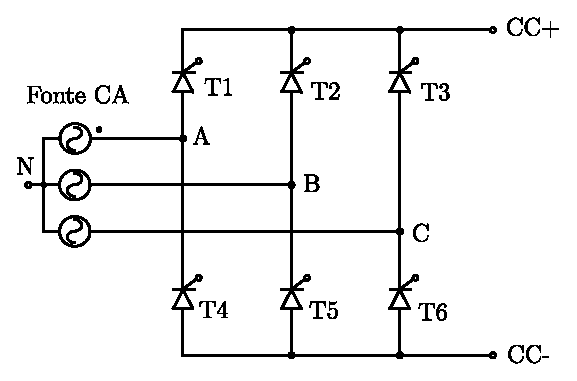
\includegraphics[width=0.5\linewidth]{figuras/NomenclaturaUtilizadaNaDisciplina}
		\caption{Nomenclatura utilizada na Disciplina.}
	\end{figure}	
	
\end{frame}



% ----------------- NOVO SLIDE --------------------------------
\section{Metodologia empregada para entender a estrutura}
%
\begin{frame}
	\frametitle{Metodologia empregada para entender a estrutura}
	\framesubtitle{Aula 06 - Retificador Trifásico de ponte completa a Tiristor}
%	
	\begin{block}{Entender cada componente}
	Antes de entender a estrutura com um todo, é necessário verificar e se certificar de como cada componente se comporta.
		%	Antes de entender o funcionamento da estrutura é preciso estabelecer corretamente a nomenclatura utilizada.
	\end{block}	
		\begin{block}{Simplificações utilizadas}
			Ter em mente as simplificações adotadas e quais fenômenos serão considerados para a análise.
			%	Antes de entender o funcionamento da estrutura é preciso estabelecer corretamente a nomenclatura utilizada.
		\end{block}	
		
		\begin{block}{Cuidar da nomenclatura utilizada}
			Ser consistente na nomenclatura utilizada para descrever a estrutura.
			%	Antes de entender o funcionamento da estrutura é preciso estabelecer corretamente a nomenclatura utilizada.
		\end{block}	
		\begin{block}{Como colocar a estrutura em operação}
			Na disciplina o foco estará na implementação via simulador.
			%	Antes de entender o funcionamento da estrutura é preciso estabelecer corretamente a nomenclatura utilizada.
		\end{block}			
%
\end{frame}
%





	
	
% ----------------- NOVO SLIDE --------------------------------


% ----------------- NOVO SLIDE --------------------------------

%\begin{frame}
%\frametitle{ABNT}
%\framesubtitle{Normas para trabalhos acadêmicos}
%
%\end{frame}

% ----------------- NOVO SLIDE --------------------------------


% ----------------- NOVO SLIDE --------------------------------
\subsection{Característica estática do tiristor ideal}
\begin{frame}
	\frametitle{Característica estática do tiristor ideal}
	%\framesubtitle{Normas para trabalhos acadêmicos}
	
	\begin{minipage}{0.45\textwidth}
		\begin{figure}
			% ensure that we have normalsize text
			\normalsize
			\centering
			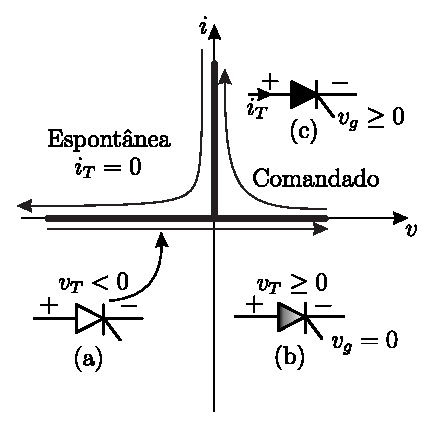
\includegraphics[width=0.9\linewidth]{figuras/TiristorCaracteristicaEstatica.eps}
			\caption{Característica estática do tiristor ideal}
			\label{fig:TiristorCaracteristicaEstatica}
		\end{figure}	
	\end{minipage}%	
	\begin{minipage}{0.65\textwidth}
		
	\begin{description}
		\item[(a):] O tiristor se encontra reversamente polarizado;
		\item[(b):] O tiristor se encontra diretamente polarizado;
		\item[(c):] O tiristor está conduzindo;
	\end{description}
	\end{minipage}
	
\end{frame}
% ----------------- NOVO SLIDE --------------------------------




% ----------------- NOVO SLIDE --------------------------------

\section{Resultados}

\begin{frame}
	\frametitle{Nomenclatura utilizada na Disciplina }
	\framesubtitle{Utilizada no livro do Prof. Ivo}
	\begin{block}{Nomenclatura}
		Antes de entender o funcionamento da estrutura é preciso estabelecer corretamente a nomenclatura utilizada.
	\end{block}	
	\begin{figure}[!h]
		\centering
		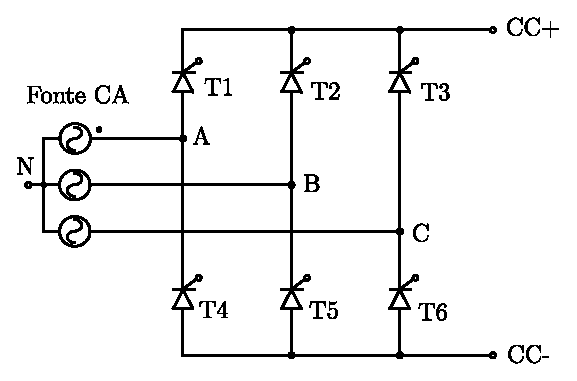
\includegraphics[width=0.5\linewidth]{figuras/NomenclaturaUtilizadaNaDisciplina}
		\caption{Nomenclatura utilizada na Disciplina.}
		\label{fig:NomenclaturaUtilizadaNaDisciplina}
	\end{figure}	
	
\end{frame}


\subsection{Nomenclatura utilizada no PSIM}
\begin{frame}
	\frametitle{Nomenclatura utilizada no PSIM}
	\framesubtitle{}
	\begin{block}{O PSIM utiliza uma nomenclatura diferente}
		Caso seja utilizado o bloco contendo a ponte retificadora a tiristor, preste atenção na nomenclatura utilizada.
	\end{block}
\begin{figure}[!h]
	\centering
	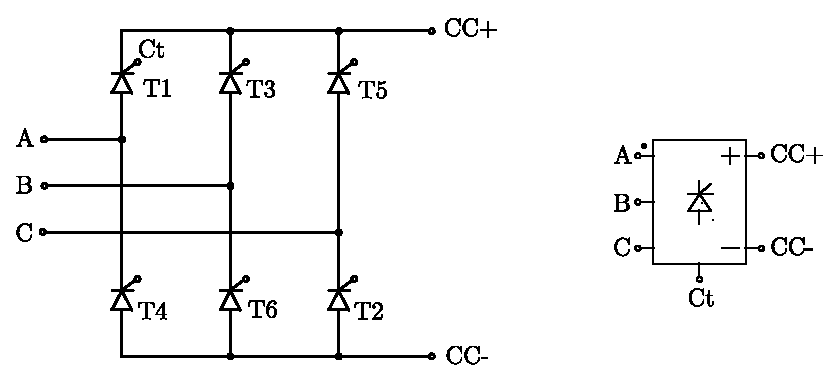
\includegraphics[width=0.7\linewidth]{figuras/PonteTiristorPSIM}
	\caption{Nomenclatura utilizada no PSIM para a ponte de Graetz a tiristor.}
	\label{fig:PonteTiristorPSIM}
\end{figure}
	
\end{frame}


\subsection{Caso particular da ponte de Graetz a tiristor}
\begin{frame}
	\frametitle{Como comandar o Tiristor?}
	\framesubtitle{Exemplo prático.}

\begin{figure}
	\centering
	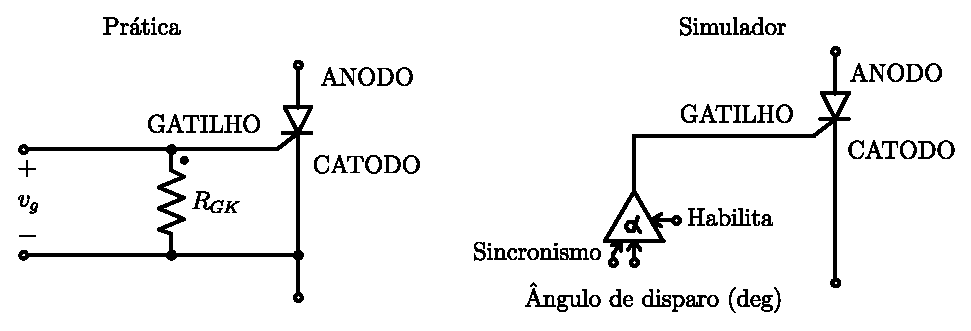
\includegraphics[width=0.8\linewidth]{figuras/TiristorPulsoGate}
	\caption{Acionamento do tiristor}
	\label{fig:TiristorPulsoGate}
\end{figure}

	\begin{block}{O sinal de gate do tiristor pode apenas ligá-lo, mas não desligá-lo.}
		\begin{description}
			\item[Sincronismo:] Transição entre reversamente polarizado para diretamente polarizado.
			\item[Ângulo de disparo:] Ângulo de disparo $\alpha$ do tiristor em graus (deg).
			%	\item[Habilita:] Se for igual a 1, habilita o controlador de pulsos do tiristor.
		\end{description}
	\end{block}
\end{frame}





\subsection{Caso particular da ponte de Graetz a tiristor}
\begin{frame}
	\frametitle{Caso particular da ponte de Graetz a tiristor}
	\framesubtitle{Obtenção do sinal de sincronismo}
	\begin{block}{Para ângulo de disparo igual a zero ($\alpha =0$)}
	A ponte retificadora a diodo é uma caso particular da ponte retificadora a tiristor.
	\end{block}
	\begin{figure}[!h]
		\centering
		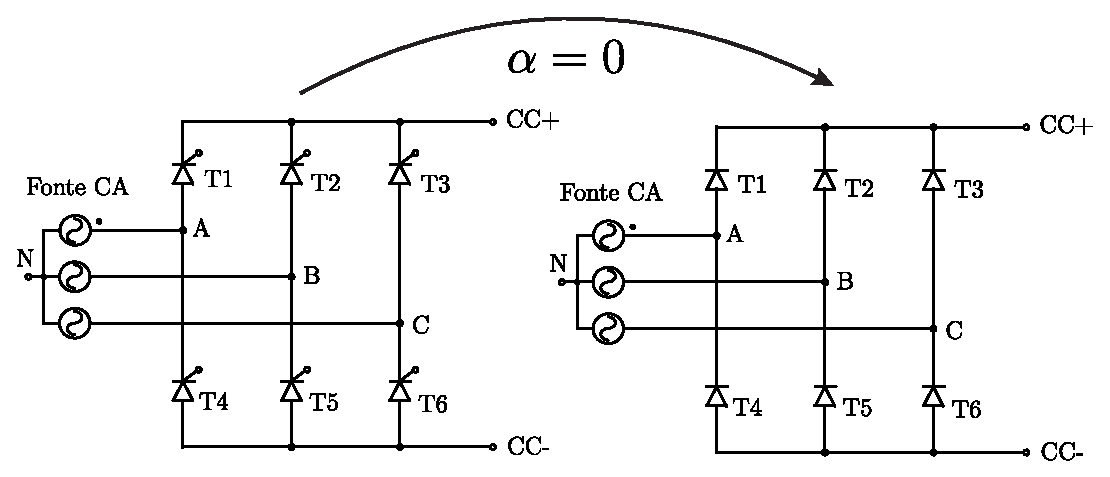
\includegraphics[width=0.85\linewidth]{figuras/TiristorCasoParticular.eps}
		\caption{Caso particular da ponte de Graetz a tiristor com $\alpha =0.$.}
	\end{figure}	
\end{frame}



\subsection{Tensão senoidal de entrada do retificador}
\begin{frame}
	\frametitle{Tensão senoidal de entrada do retificador}
%	\framesubtitle{Obtenção do sinal de sincronismo}
	\begin{block}{Sistema trifásico utilizado}
		Determinada a topologia retificadora, o próximo passo é saber o comportamento da fonte de entrada CA.
	\end{block}


\begin{eqnarray}
{v_{an}} &=& {V_{ll,{\textrm{rms}}}}\sqrt {\frac{2}{3}} \sin \left( {\omega t} \right)\\
{v_{bn}} &=& {V_{ll,{\textrm{rms}}}}\sqrt {\frac{2}{3}} \sin \left( {\omega t - \frac{{2\pi }}{3}} \right)\\
{v_{cn}} &=& {V_{ll,{\textrm{rms}}}}\sqrt {\frac{2}{3}} \sin \left( {\omega t + \frac{{2\pi }}{3}} \right)
\end{eqnarray}	
\end{frame}




\begin{frame}
	\frametitle{Tensão senoidal de entrada do retificador}
		\framesubtitle{Tensões trifásicas aplicadas ao retificador}
\begin{figure}
	\centering
	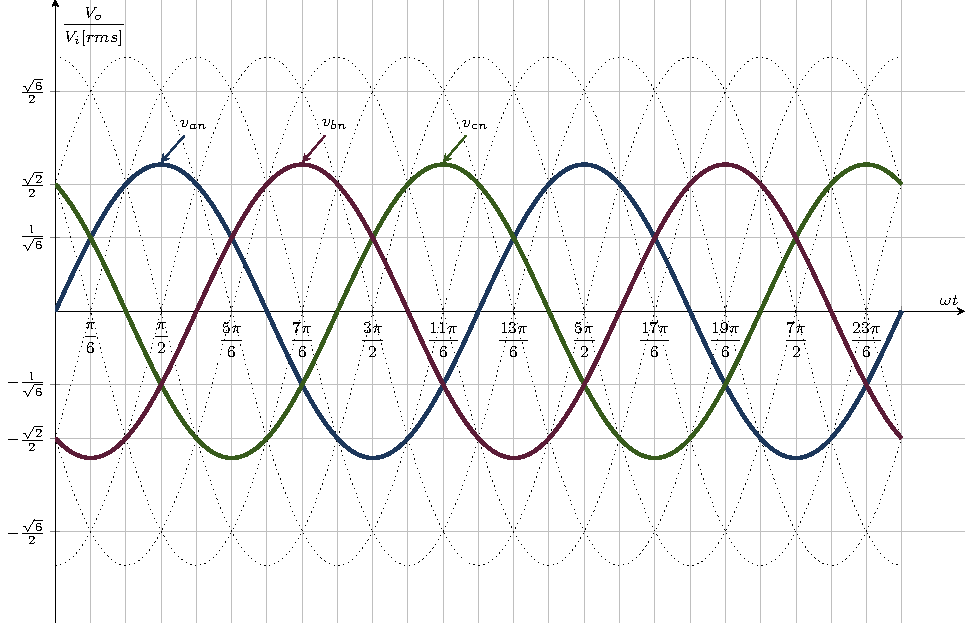
\includegraphics[width=0.8\linewidth]{figuras/SenosDrawVabcnSEQn}
	\caption{Tensão de entrada do retificador trifásico a tiristor}
	\label{fig:SenosVabcn}
\end{figure}	
\end{frame}

\begin{frame}
	\frametitle{Tensão senoidal de linha na entrada do retificador}
	\framesubtitle{Tensões trifásicas de linha aplicadas ao retificador}
	
	\begin{figure}
\centering
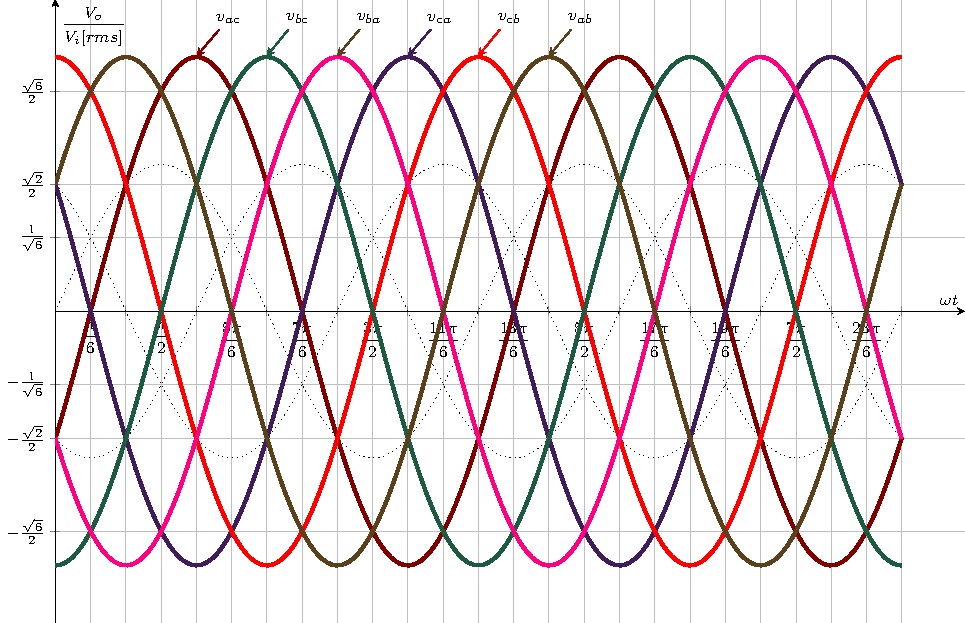
\includegraphics[width=0.7\linewidth]{figuras/SenosDrawSEQnTensoesLinha}
\caption{Tensões de linha entrada do retificador trifásico a tiristor.}
\label{fig:SenosDrawSEQnTensoesLinha}
\end{figure}
	
\end{frame}




\subsection{Polarização do tiristor T1 e T4}
\begin{frame}
	\frametitle{Polarização do tiristor T1}
	\framesubtitle{A inversão de fase se aplica ao tiristor T4}

O primeiro braço esta conectada a fonte $v_{an}$, assim sendo devemos observar as tensões $v_{ab}$ e $v_{ac}$.
\begin{figure}
	\centering
	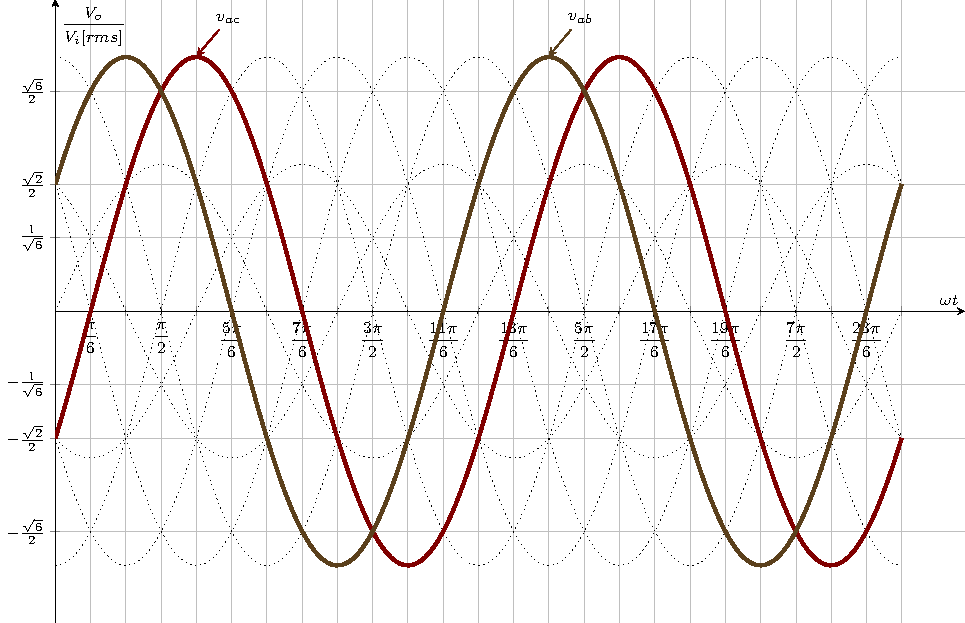
\includegraphics[width=0.6\linewidth]{figuras/SenosDrawSEQnT1T4}
	\caption{Tensões $v_{ab}$ e $v_{ac}$}
	\label{fig:SenosDrawSEQnT1T4}
\end{figure}
	
\end{frame}

\subsection{Configurações possíveis T1 e T4}

\begin{frame}
	\frametitle{Configurações possíveis para polarização do tiristor T1}
	\framesubtitle{Sem roda livre}
	
	\begin{minipage}{0.5\textwidth}\centering
		Condição:\\ $v_{ac} \ge $ demais tensões.
		\begin{figure}
			\centering
			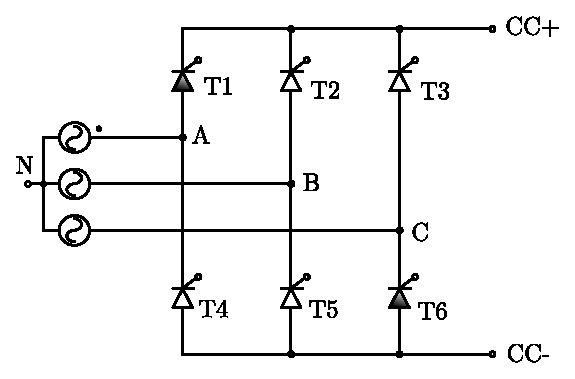
\includegraphics[width=0.9\linewidth]{figuras/GraetzTiristorT1T6}
			\caption{Tiristores T1 e T6 estão diretamente polarizados.}
			\label{fig:GraetzTiristorT1T6}
		\end{figure}	
	\end{minipage}%	
	\begin{minipage}{0.5\textwidth}\centering
		Condição:\\ $v_{ab} \ge $ demais tensões.
		\begin{figure}
			\centering
			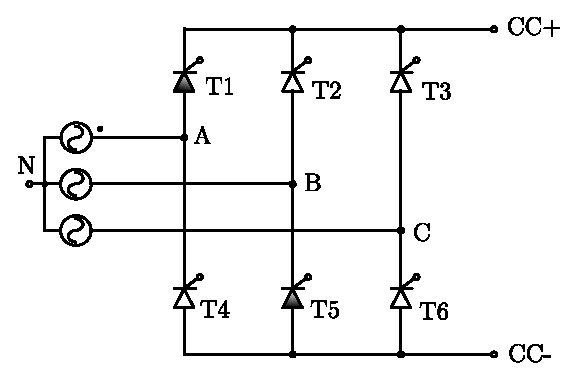
\includegraphics[width=0.9\linewidth]{figuras/GraetzTiristorT1T5}
			\caption{Tiristores T1 e T5 estão diretamente polarizados.}
			\label{fig:GraetzTiristorT1T5}
		\end{figure}
		
	\end{minipage}
	
\end{frame}



\subsection{Polarização do tiristor T2 e T5}
\begin{frame}
	\frametitle{Polarização do tiristor T2}
	\framesubtitle{A inversão de fase se aplica ao tiristor T5}
	
O segundo braço esta conectada a fonte $v_{bn}$, assim sendo devemos observar as tensões $v_{ba}$ e $v_{bc}$
\begin{figure}
	\centering
	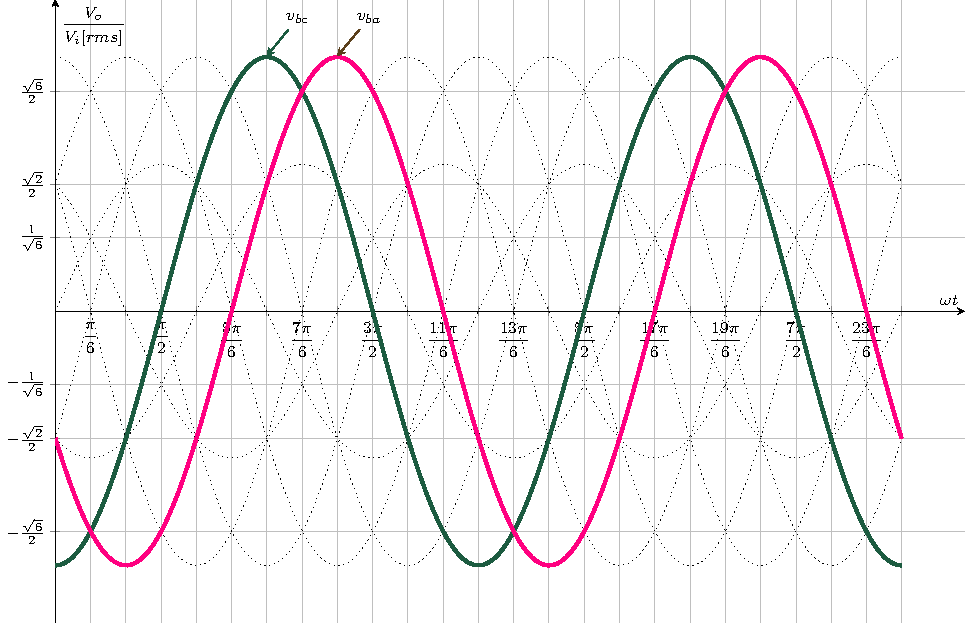
\includegraphics[width=0.6\linewidth]{figuras/SenosDrawSEQnT2T5}
	\caption{Tensões  $v_{ba}$ e $v_{bc}$}
	\label{fig:SenosDrawSEQnT2T5}
\end{figure}
\end{frame}


\subsection{Configurações possíveis T2 e T5}

\begin{frame}
	\frametitle{Configurações possíveis para polarização do tiristor T2}
	\framesubtitle{Sem roda livre}
	
	\begin{minipage}{0.5\textwidth}\centering
		Condição:\\ $v_{ba} \ge $ demais tensões.
		\begin{figure}
			\centering
			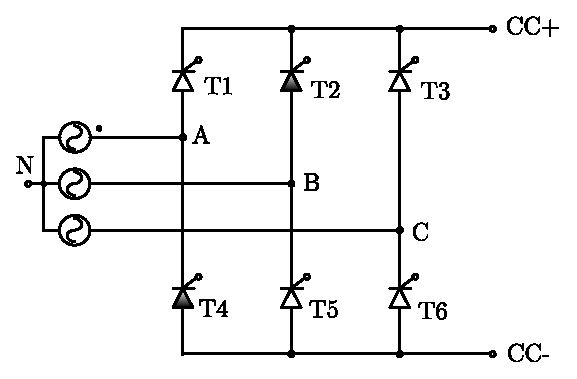
\includegraphics[width=0.9\linewidth]{figuras/GraetzTiristorT2T4}
			\caption{Tiristores T2 e T4 estão diretamente polarizados.}
			%			\label{fig:GraetzTiristorT1T6}
		\end{figure}	
	\end{minipage}%	
	\begin{minipage}{0.5\textwidth}\centering
		Condição:\\ $v_{bc} \ge $ demais tensões.
		\begin{figure}
			\centering
			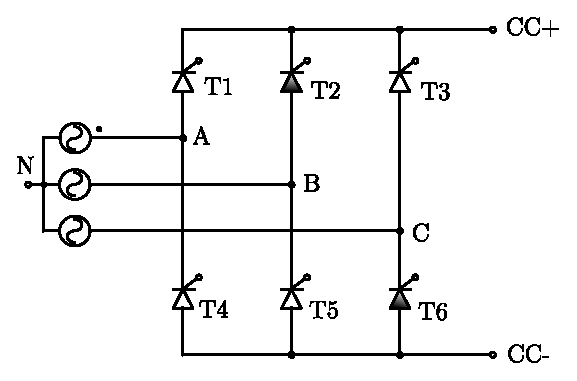
\includegraphics[width=0.9\linewidth]{figuras/GraetzTiristorT2T6}
			\caption{Tiristores T2 e T6 estão diretamente polarizados.}
			%			\label{fig:GraetzTiristorT1T5}
		\end{figure}		
	\end{minipage}	
\end{frame}

\subsection{Polarização do tiristor T3 e T6}
\begin{frame}
	\frametitle{Polarização do tiristor T3}
	\framesubtitle{A inversão de fase se aplica ao tiristor T6}
	
O terceiro braço esta conectada a fonte $v_{cn}$, assim sendo devemos observar as tensões $v_{ca}$ e $v_{cb}$
\begin{figure}
	\centering
	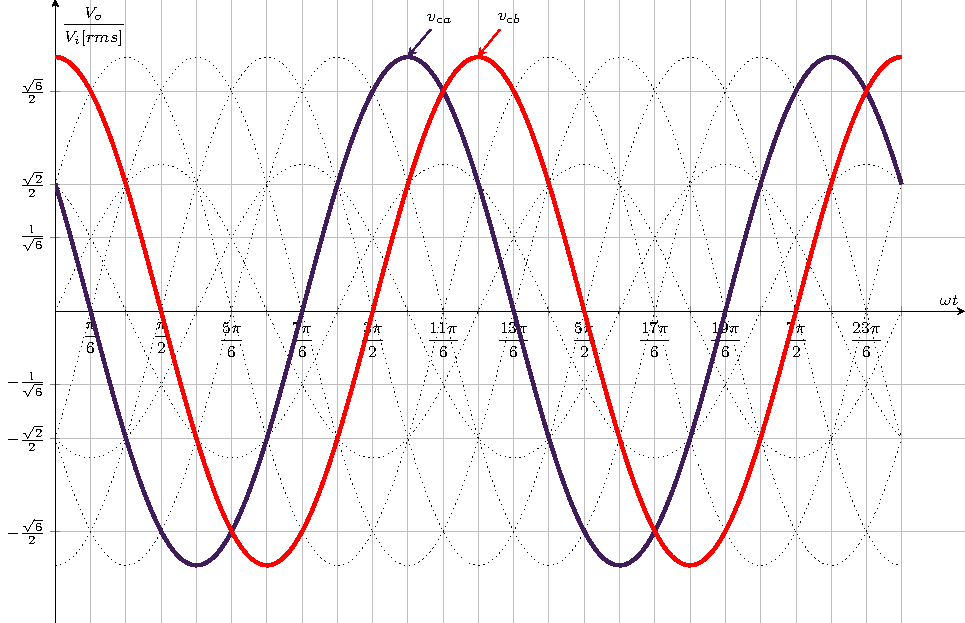
\includegraphics[width=0.6\linewidth]{figuras/SenosDrawSEQnT3T6}
	\caption{Tensões  $v_{ca}$ e $v_{cb}$}
	\label{fig:SenosDrawSEQnT3T6}
\end{figure}

\end{frame}




\subsection{Configurações possíveis T3 e T6}
\begin{frame}
	\frametitle{Configurações possíveis para polarização do tiristor T3}
	\framesubtitle{Sem roda livre}
	
	\begin{minipage}{0.5\textwidth}\centering
		Condição:\\ $v_{ca} \ge $ demais tensões.
		\begin{figure}
			\centering
			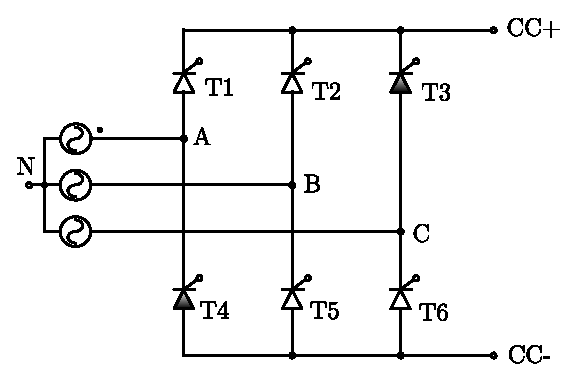
\includegraphics[width=0.9\linewidth]{figuras/GraetzTiristorT3T4}
			\caption{Tiristores T3 e T4 estão diretamente polarizados.}
			%			\label{fig:GraetzTiristorT1T6}
		\end{figure}	
	\end{minipage}%	
	\begin{minipage}{0.5\textwidth}\centering
		Condição:\\ $v_{cb} \ge $ demais tensões.
		\begin{figure}
			\centering
			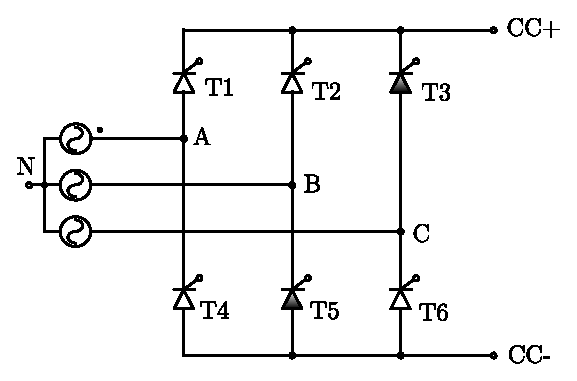
\includegraphics[width=0.9\linewidth]{figuras/GraetzTiristorT3T5}
			\caption{Tiristores T3 e T5 estão diretamente polarizados.}
			%			\label{fig:GraetzTiristorT1T5}
		\end{figure}		
	\end{minipage}	
\end{frame}




\subsection{Operação com angulo zero}
\begin{frame}
	\frametitle{Operação com ângulo de disparo nulo ($\alpha=0$)}
	\framesubtitle{Operação similar ao retificado trifásico a diodo}
	
\begin{figure}
	\centering
	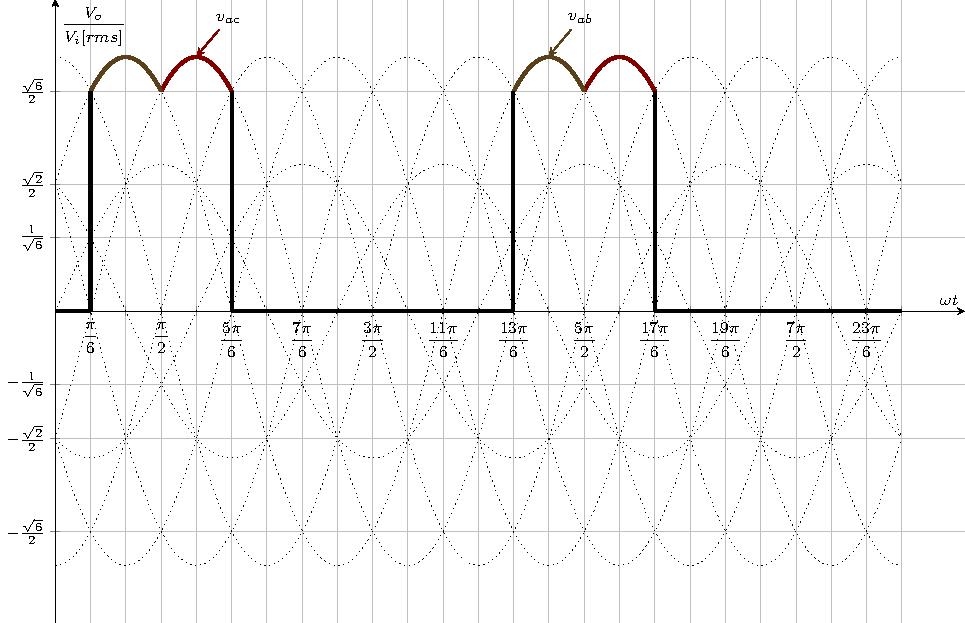
\includegraphics[width=0.7\linewidth]{figuras/SenosDrawSEQnT1alpha0}
	\caption{Caso particular com ângulo de disparo nulo.}
	\label{fig:SenosDrawSEQnT1alpha0}
\end{figure}

\end{frame}



\subsection{Operação com 30 graus de disparo}
\begin{frame}
	\frametitle{Operação com ângulo de disparo  ($\alpha=30^o$)}
	\framesubtitle{Corrente no tiristor T1, operação com carga resistiva}
	
	\begin{figure}
\centering
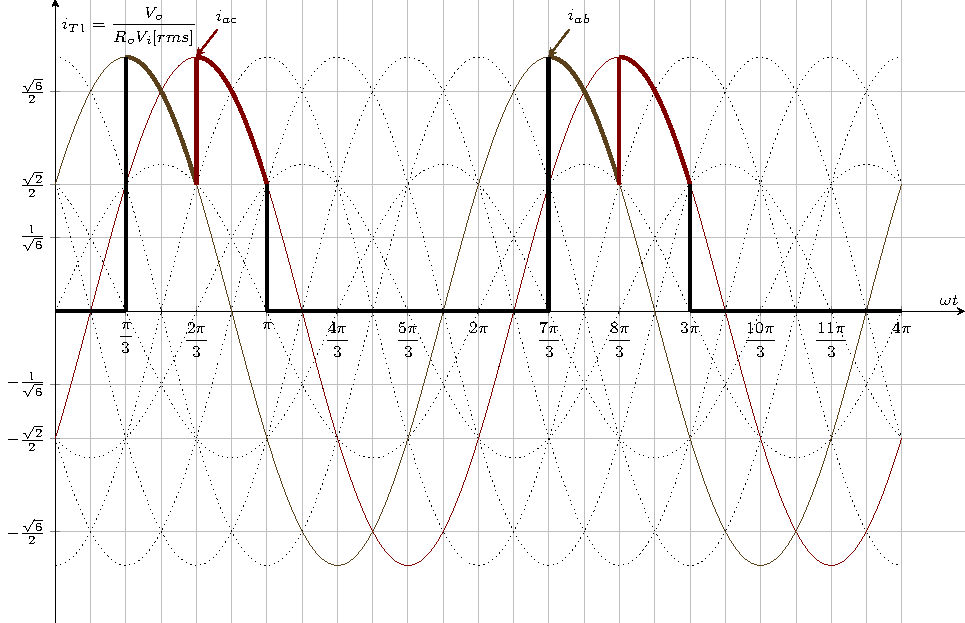
\includegraphics[width=0.7\linewidth]{figuras/SenosDrawSEQnT1alpha30}
\caption{Caso particular com ângulo de disparo $\alpha =$ 30 graus}
\label{fig:SenosDrawSEQnT1alpha30}
\end{figure}


\end{frame}


\subsection{Operação com 60 graus de disparo}
\begin{frame}
	\frametitle{Operação com ângulo de disparo  ($\alpha=60^o$)}
	\framesubtitle{Corrente no tiristor T1, operação com carga resistiva}
	
	\begin{figure}
		\centering
		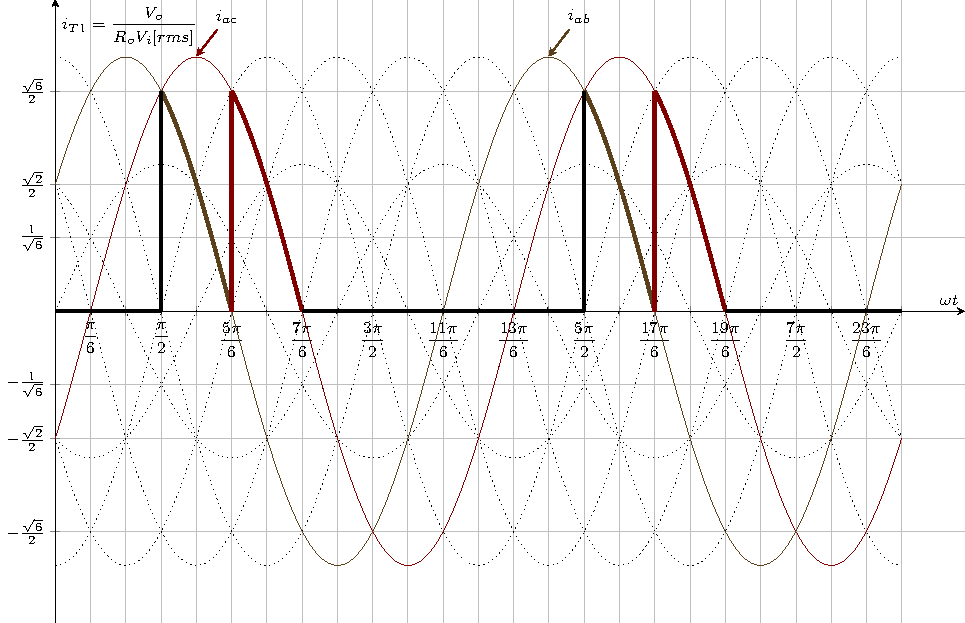
\includegraphics[width=0.7\linewidth]{figuras/SenosDrawSEQnT1alpha60}
		\caption{Caso particular com ângulo de disparo $\alpha =$ 60 graus}
		\label{fig:SenosDrawSEQnT1alpha60}
	\end{figure}	
\end{frame}


\subsection{Operação com 90 graus de disparo}
\begin{frame}
	\frametitle{Operação com ângulo de disparo ($\alpha=90^o$)}
	\framesubtitle{Corrente no tiristor T1, operação com carga resistiva}
	
	\begin{figure}
		\centering
		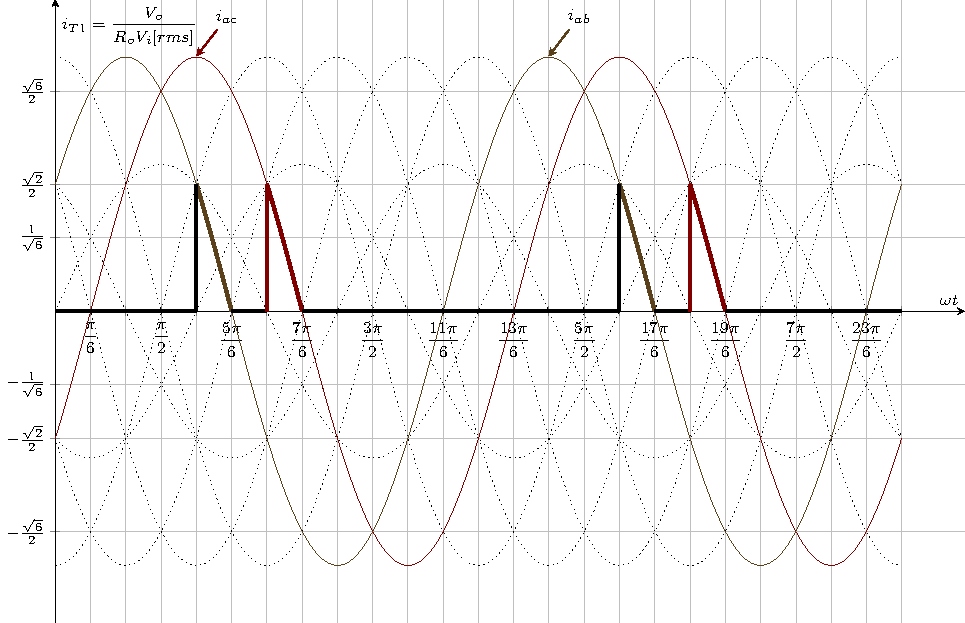
\includegraphics[width=0.7\linewidth]{figuras/SenosDrawSEQnT1alphaR90}
		\caption{Caso particular com ângulo de disparo $\alpha =$ 90 graus}
		\label{fig:SenosDrawSEQnT1alpha90}
	\end{figure}	
\end{frame}


\subsection{Regiões de operação}
\begin{frame}
	\frametitle{Regiões de operação com carga resistiva}
	\framesubtitle{Definida pelas condições de continuidade.}
	\begin{block}{Condução contínua}
		 Para $ 0 \le \alpha \le \frac{\pi}{3}$ ou $ 0 \le \alpha \le 60^o$ a condução é contínua.
	\end{block}
		\begin{block}{Condução descontínua}
			Para $ \frac{\pi}{3} \le \alpha \le \frac{2\pi}{3}$ ou $ 0 \le \alpha \le 120^o$ a condução é contínua.
		\end{block}
%	Para /3 <  < 2/3, a condução é descontínua
\end{frame}








\subsection{Operação com 90 graus de disparo e carga indutiva}
\begin{frame}
	\frametitle{Operação com ângulo de disparo ($\alpha=90^o$)}
	\framesubtitle{Corrente no tiristor T1, operação com carga resistiva indutiva}
	
	\begin{figure}
		\centering
		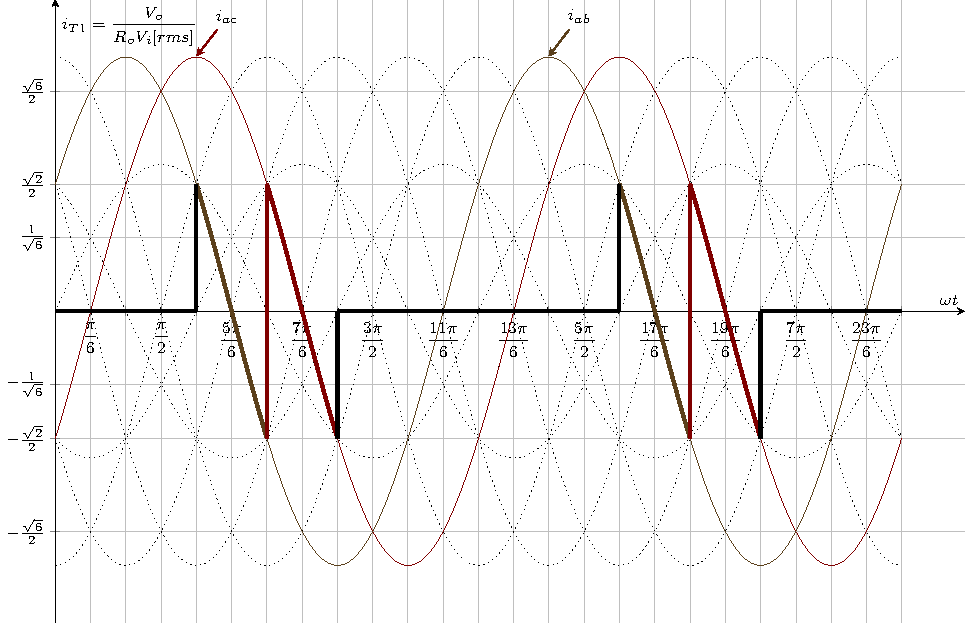
\includegraphics[width=0.7\linewidth]{figuras/SenosDrawSEQnT1alphaRL}
		\caption{Caso particular com ângulo de disparo $\alpha =$ 90 graus}
		\label{fig:SenosDrawSEQnT1alphaRL}
	\end{figure}	
\end{frame}


\subsection{Regiões de operação}
\begin{frame}
	\frametitle{Regiões de operação com carga resistiva}
	\framesubtitle{Definida pela tensão média na carga.}
	\begin{block}{Operação como retificador}
		Para $ 0 \le \alpha \le \frac{\pi}{2}$ ou $ 0 \le \alpha \le 90^o$ a tensão média na carga é positiva.
	\end{block}
	\begin{block}{Operação como inversor não autônomo}
		Para $ \frac{\pi}{2} \le \alpha \le \pi$ ou $ 0 \le \alpha \le 180^o$ a tensão média na carga é negativa.
	\end{block}
	%	Para /3 <  < 2/3, a condução é descontínua
\end{frame}


\subsection{Dúvidas??}
\begin{frame}
	\frametitle{Dúvidas??}
	\framesubtitle{Retificador trifásico de onda completa a tiristor.}
	\begin{block}{Qual tal simularmos a estrutura para verificar a validade do que foi apresentado?}
		O software utilizado será o PSIM, que pode ser encontrado no link:
		\url{http://powersimtech.com/products/psim/}
	\end{block}

\end{frame}




\subsection{Valores médios de tensão na carga}
\begin{frame}
	\frametitle{Valores médios das tensões}
	\framesubtitle{Definida pelas condições de continuidade.}
		\begin{block}{Ângulo de disparo nulo $\alpha = 0$}
		   Operando como retificador a diodo.
		\end{block}
			\begin{equation}
				{V_{Lmed}} = 2,34\,{V_o}
			\end{equation}
	
	\begin{block}{Condução contínua}
		Para $ 0 \le \alpha \le \frac{\pi}{3}$ ou $ 0 \le \alpha \le 60^o$ a condução é contínua.
	\end{block}
	
	
	\begin{equation}
     {V_{Lmed}} = 2,34\,{V_o}\,\cos \,\alpha 
	\end{equation}

	%	Para /3 <  < 2/3, a condução é descontínua
\end{frame}




\subsection{Valores médios de tensão na carga }
\begin{frame}
	\frametitle{Valores médios das tensões com carga resistiva}
	\framesubtitle{Definida pelas condições de continuidade.}

	\begin{block}{Condução descontínua com carga resistiva}
		\begin{equation}
		{V_{Lmed}} = 2,34\,{V_{o}}\,\left[ {1 + \cos \,\left( {\frac{\pi }{3} + \alpha } \right)} \right]
		\end{equation}
	\end{block}
	%	Para /3 <  < 2/3, a condução é descontínua
	
	

	
	
\end{frame}





\subsection{Valores médios de tensão na carga }
\begin{frame}
	\frametitle{Valores médios das tensões com carga resistiva indutiva}
	\framesubtitle{Definida pelas condições de continuidade.}
	
	
	\begin{block}{Condução descontínua com carga resistiva indutiva}
		\begin{equation}
		{V_{Lmed}} = 2,34\,{V_o}\,\cos \,\alpha 
		\end{equation}
	\end{block}
	
	
\end{frame}


\section{Referências}

% --- O comando \allowframebreaks ---
% Se o conteúdo não se encaixa em um quadro, a opção allowframebreaks instrui 
% beamer para quebrá-lo automaticamente entre dois ou mais quadros,
% mantendo o frametitle do primeiro quadro (dado como argumento) e acrescentando 
% um número romano ou algo parecido na continuação.

\begin{frame}[allowframebreaks]{Referências}
%\bibliography{abntex2-modelo-references}



\begin{thebibliography}{}
	
	\bibitem{IvoBarbi2006} I. Barbi, “Eletrônica de Potência”. Edição do Autor, 6a Edição Florianópolis,
	2006.
	
	\bibitem{Pelly} Pelly, B. R.. Thyristor Phase-controlled Converters and Cycloconverters - Ed. John Wiley \& Sons, New York, 1971.
	
	\bibitem{HBD855} Semiconductors, On. "Thyristor Theory and Design Considerations." HBD855/D (2005): 11.
	
	\bibitem{PSIM} Mourant, R. R. "PSIM User's Manual." Micro Simulation, Boston, MA (1983).
	%	
	
\end{thebibliography}
\end{frame}

% ----------------- FIM DO DOCUMENTO -----------------------------------------
\end{document}
